\documentclass[a4paper]{article}
\usepackage{labreport}

\begin{document}

\section{Objective}
The objective is to analyze a circuit and measure the real values to validate the calculated values \cite{UNCC-ECE-Dept:2023}.
\section{Equipment Used}

\begin{itemize}
    \item Digital Multimeter
    \item DC Power Supply
    \item Resistors: $470\Omega$, $1K\Omega$ (2), $5.1k\Omega$, $10k\Omega$ 
\end{itemize}

\section{Experiment Setup}
Prelab to fill in the table\\
\begin{enumerate}
    \item Use mesh analysis to calculate: $I_{A}$, $I_{B}$, and $I_{C}$ \cite{UNCC-ECE-Dept:2023}.
    \item Use the mesh currents to calculate the current through and voltage across each resistor \cite{UNCC-ECE-Dept:2023}.
    \item Use the method of superposition to calculate the current through and voltage across each resistor \cite{UNCC-ECE-Dept:2023}.
    \item Construct the circuit in a modeling software as seen in Figure 8-2 and record the results \cite{UNCC-ECE-Dept:2023}. 
\end{enumerate}

Lab to measure values\\
\begin{enumerate}
    \item Construct the circuit in Figure 8-1 and record the values in the color code value on the resistors \cite{UNCC-ECE-Dept:2023}.
    \begin{figure}[H]\label{fig8-1}
        \begin{center}
            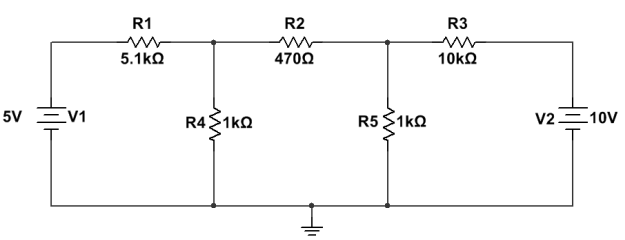
\includegraphics{fig8-1}\\
            \small\textbf{Figure 8-1: Circuit for testing \cite{UNCC-ECE-Dept:2023}}
        \end{center}
    \end{figure}
    \item Measure the voltage and current across and through each resistor for the values \cite{UNCC-ECE-Dept:2023}.
    \item For the measured values of Table 8-2 use the current across $R_{1}$, $R_{2}$, $R_{3}$ \cite{UNCC-ECE-Dept:2023}.   
\end{enumerate}
\section{Results}

\begin{center}
    \small\textbf{Table 8-1: Resistors Values \cite{UNCC-ECE-Dept:2023}}
    \begin{tabular}{|p{3 cm}|p{3cm}|p{3 cm}|p{3 cm}|}
        \hline
        Resistance & Measured $(K\Omega)$ & Color Code $(K\Omega)$ & Error (\%) \\
        \hline
        $R_{1}$ & $5.047 k\Omega$ & $5.1k\Omega$ & 1.0392 \% \\
        \hline
        $R_{2}$ & $467.5 \Omega$ & $470\Omega$& .5319\% \\
        \hline
        $R_{3}$ & $9.935 k\Omega$ & $10 k\Omega$& .65\% \\
        \hline
        $R_{4}$ & $.999 k\Omega$ & $1 k\Omega$& .1\% \\
        \hline
        $R_{5}$ & $.997 k\Omega$ & $1 k\Omega$ & .3\% \\
        \hline
    \end{tabular}
\end{center}

\begin{center}
    \small\textbf{Table 8-2: Mesh Currents \cite{UNCC-ECE-Dept:2023}}
    \begin{tabular}{|p{3 cm}|p{3cm}|p{3 cm}|p{3 cm}|}
        \hline
        Current & Measured (mA) & Calculated (mA) & Error (\%) \\
        \hline
        $I_{A}$ & .806 mA & .813 mA & .861\%  \\
        \hline
        $I_{B}$ & .043 mA & .0404 mA & 5.581\% \\
        \hline
        $I_{C}$ & .910 mA & .913 mA & .329\% \\
        \hline
    \end{tabular}
\end{center}

\begin{center}
    \small\textbf{Table 8-3: Resistors Voltages \cite{UNCC-ECE-Dept:2023}}
    \begin{tabular}{|p{2 cm}|p{2cm}|p{2 cm}|p{2 cm}|p{2 cm}|p{2 cm}|}
        \hline
         & Measured & Mesh Method & Nodal Analysis & Superposition & Simulation \\
        \hline
        $V_{R1}$ & 4.14 V & 4.1463 V & 4.43368 V & 4.1466 V & 4.147 V \\
        \hline
        $V_{R2}$ & .021 V & .018988 V & .018 V & .01897 V & .01897 V \\
        \hline
        $V_{R3}$ & 9.123 V & 9.13 V & 9.128 V & 9.158 V & 9.128 V \\
        \hline
        $V_{R4}$ .852 V & & .854 V & .853 V & .853 V & .8534 V \\
        \hline
        $V_{R5}$ & .873 V & .8721 V & .872 V & .873 V & .8724 V \\
        \hline
    \end{tabular}
\end{center}

\begin{center}
    \small\textbf{Table 8-4: Resistors Current \cite{UNCC-ECE-Dept:2023}}
    \begin{tabular}{|p{2 cm}|p{2cm}|p{2 cm}|p{2 cm}|p{2 cm}|p{2 cm}|}
        \hline
         & Measured & Mesh Method & Nodal Analysis & Superposition & Simulation \\
        \hline
        $I_{R1}$ & .803 mA  & .813 mA & .8131 mA & .81305 mA &.8131 mA \\
        \hline
        $I_{R2}$ & .043 mA & .0406 mA & .0404 mA & .04037 mA  & .04034 mA\\
        \hline
        $I_{R3}$ & .911 mA & .913 mA & .9128 mA & .91276 mA & .9128 mA \\
        \hline
        $I_{R4}$ & .825 mA & .8536 mA & .853 mA &  .853 mA & .8534 mA\\
        \hline
        $I_{R5}$ & .834 mA & .8271 mA & .872 mA & .873 mA & .8724 mA\\
        \hline
    \end{tabular}
\end{center}

\begin{center}
    \begin{figure}[H]\label{fig8-2}
        \begin{center}
            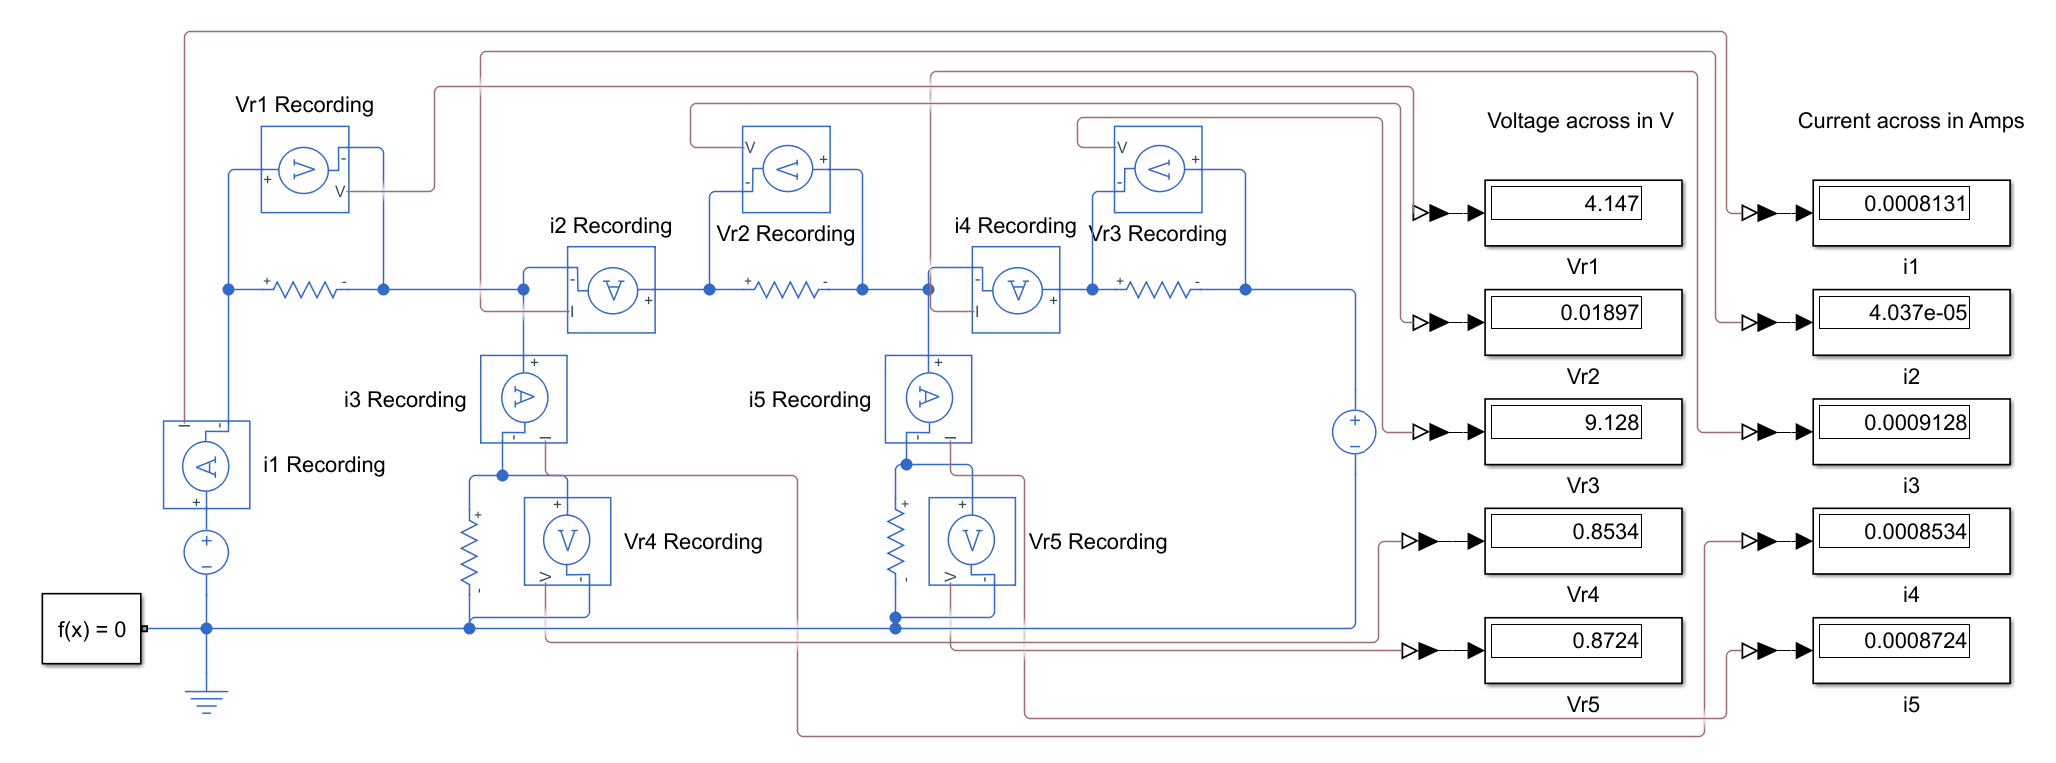
\includegraphics[width = 16 cm]{Figure_8-1}\\
            \small\textbf{8-2: Simulated model of the circuit in Figure 8-1}\\    
        \end{center}
    \end{figure}
\end{center}
\section{Conclusion}

Each method of calculation will introduce error due to its assumption of ideal conditions. Furthermore, each almost all methods of calculations
will give similar value but will vary in precision.


\bibliography{references}
\bibliographystyle{plain}



\end{document}